\chapter{Localizing Group Differences over
Covariance Trajectories}\label{sec:covtraj}

Feature selection has become a core problem with the increase in dimensionality of learning problems.
Identifying and exploiting conditional independencies within data enables previously intractable problems to be solved,
and this chapter focuses on one particular angle along this direction.
% Multivariate data analysis exploiting the conditional independence structure between features or covariates using 
% undirected graphical models is now standard within any data analysis toolbox. 
When data are multivariate Gaussian, the zeros in the inverse covariance (precision) matrix give conditional independences 
among the variables \citep{lauritzen1996graphical}. 
Further, if the precision matrix is sparse, we can
derive dependencies between features when the data are high-dimensional and/or the number of measurements are small. 
The estimation of a graphical model
has been extensively studied
%in statistics and machine learning,
and a rich literature is available describing 
its statistical and algorithmic properties \citep{koller2009probabilistic,jordan1998learning}. 
For instance, the so-called \textit{graphical lasso} formulation uses an $\ell_1$-norm penalty on the 
precision matrix and is widely used, and consistency properties 
in the large $p$ regime \citep{cai2011constrained,friedman2008sparse,yuan2010high} are now well understood.
These formulations have also been extended to various transformations of Gaussian distributions (e.g., non-paranormal)
%, where the 
using rank statistics \citep{liu2009nonparanormal,xue2012regularized,liu2012high}.
%are a consistent estimator of 
%the precision matrix nonzero pattern 

{\em Coupled and Temporal Graphical Models.} 
%In various situations,
Often, data come from two (or more) disparate sources or multiple timepoints.
Within the last few years, a few proposals have 
described strategies for linking the sparsity patterns of multiple graphical models, e.g., using a fused lasso 
penalty \citep{danaher2014joint} \citep{yang2015fused}. Observe that 
%these ideas assume that the two (or more) models share a similar structure; 
if the data sources correspond to {\em longitudinal} acquisitions, we should expect 
the `structure' to gradually evolve.
%, which is discouraged in direct applications of the above idea. 
%in the case where the model is changing such a construction would not allow for identification of the evolving graph structure. 
% Several authors have offered generalizations to address this problem: \citep{zhou2010time} removes the assumption
% that each graph is independent and structurally `close'.
% Instead, \citep{zhou2010time} can be thought of as a growth model \citep{mcardle2000introduction} defined on these structures: they show how non-identically distributed graphs can be learned over time. 
% Recently, the nonparametric procedure in \citep{qiu2015joint} extends these ideas
% %via means
% to handle multiple sources, each with multiple samples.

The ideas in the literature so far to ``couple'' multiple graphical model estimation modules are mostly nonparametric \citep{zhou2010time, mcardle2000introduction,qiu2015joint}. 
While such a formulation offers benefits, in many estimation problems, 
parametric models may 
%require fewer samples (better convergence rates) and possibly, 
be more convenient for downstream statistical analysis,
particularly for hypothesis testing \citep{hardle1993comparing,geer2000empirical,roehrig1988conditions}.
% Given that the topic of \textit{coupled} graphical models, by itself, is fairly recent, algorithms for {\em parametric estimation} of 
% temporal or coupled Gaussian graphical models have not yet been heavily studied. 
\begin{figure*}[t]
  \centering
  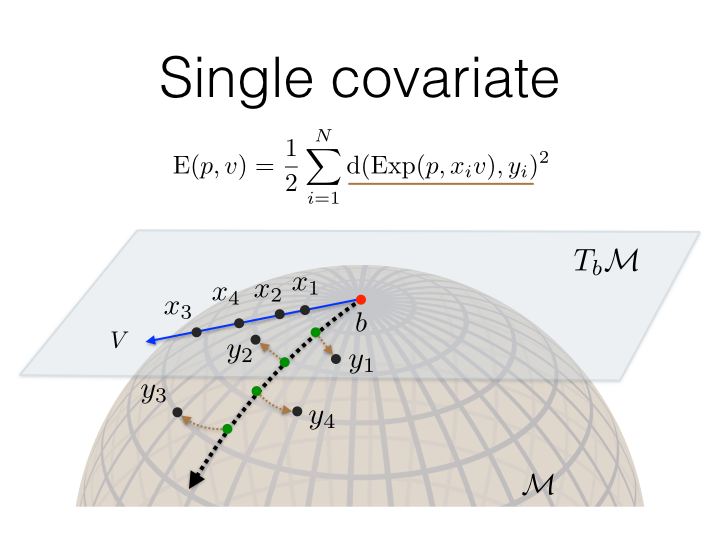
\includegraphics[width=0.49\textwidth,trim={10 40 10 220},clip]{chap2/MGLM1.png}
  %
    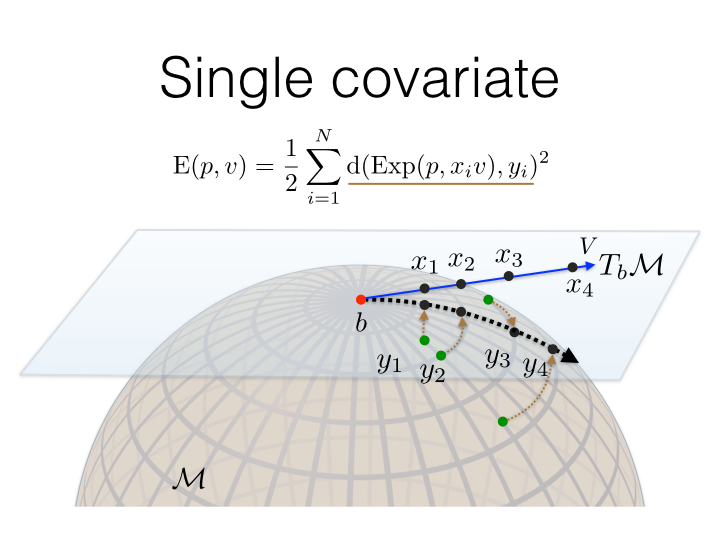
\includegraphics[width=0.49\textwidth,trim={10 40 10 220},clip]{chap2/MGLM2.png}
  \caption{\small\label{fig:manifold}Group-wise MMGLM: The left and right figures represent two linear models on the $\SPD(p)$ manifold. Points $x_i$ in the tangent space are our covariate or predictor, and points $y_i$ in the manifold space represent $\SPD(p)$ matrices. In our regression setting, we wish to minimize the error (brown curves) between the estimation and the sample points. Because each linear model has a different base point, the trajectories cannot be directly compared as in the Euclidean setting.}
\end{figure*}

%Part of the reason is the difficulty of 
This will involve parameterizing {\em trends} in the highly structured nature of the `response' variable ($\SPD$ matrices). 
%In contrast, w
Parametric formulations for manifold-valued data {\em have} been proposed recently \citep{hjkimcvpr2014,cornea2016regression}. %, albeit only in the 
%context of regression models and dictionary learning \citep{xie2013nonlinear}. 
%This result is relevant --- b
Because $\SPD$ matrices form a Riemannian manifold, algorithms
that estimate a parametric model respecting the underlying Riemannian metric are more suitable in many applications as opposed to assuming a Euclidean metric 
on positively or negatively curved spaces \citep{xie2010statistical, fletcher2007riemannian, jayasumanakernel}. We will make a few simple modifications 
(for efficiency purposes) to such algorithms and make use of the estimated parameters for follow-up analysis. 

%Unfortunately, their deployment for the $\SPD$ may not always be trivial.

{\em Finding Group-wise Differences.} Assuming that we have a black-box procedure to estimate a parametric model on the $\SPD$ manifold available, 
in many tasks, such an estimation is merely a segue to other analyses designed to answer scientifically meaningful questions. 
For example, we are often interested in asking whether the temporally coupled model estimated using the procedure above differs 
in meaningful ways {\em across} groups induced by a stratification or dichotomous variable (e.g., gender or disease). For instance, is the `slope' in structured response space statistically different 
across education level or body mass index? 
%in if this model differs significantly across two groups.
While the body of work for graphical model estimation is mature, the literature describing hypothesis tests in this
regime \citep{diffnet,belilovsky2015hypothesis}
is sparse at best.

Given that such questions are simpler to answer with alternative schemes (with assumptions on the distributional properties of the data), e.g., structural equation modeling, 
latent growth models and so on \citep{ullman2003structural, mcardle2000introduction}, it seems that 
the unavailability of such tools is limiting the adoption of such ideas in a broader 
cross-section of science. We will seek to address this gap. 

\begin{figure}[h]
    \centering
    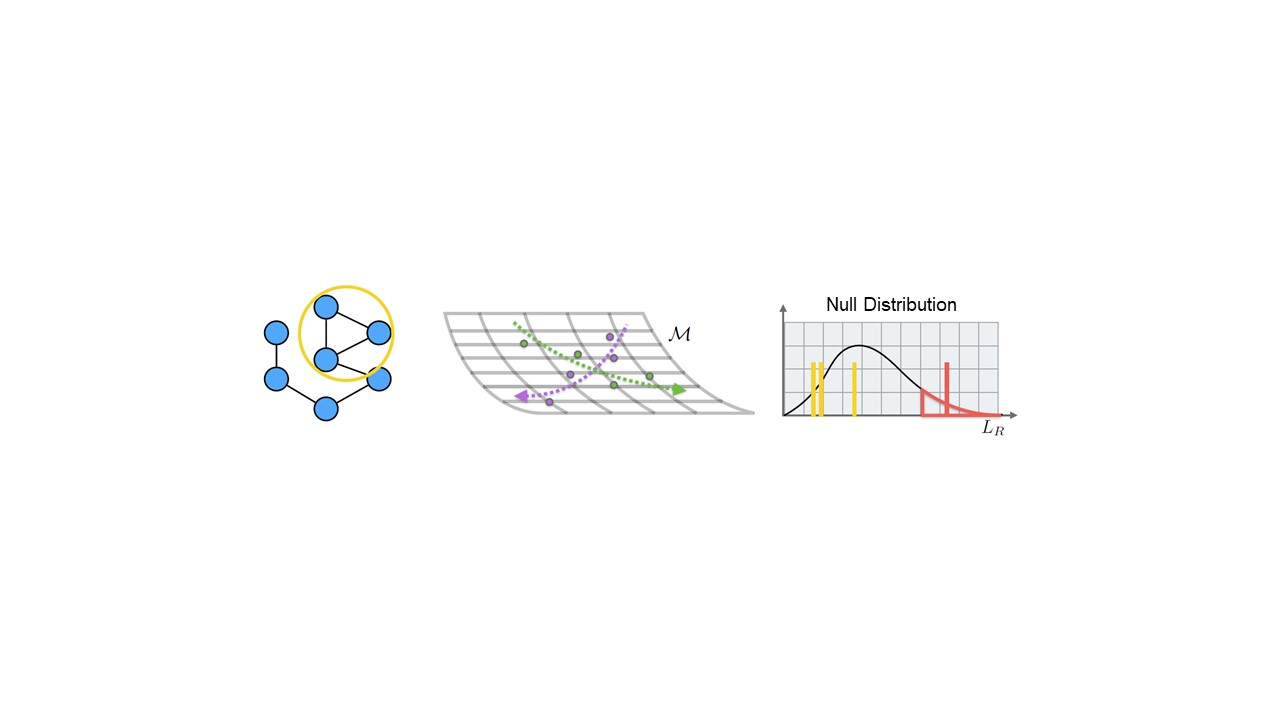
\includegraphics[width=\columnwidth,trim={6.5cm 7.5cm 6.5cm 7.5cm},clip]{chap2/method.jpg}
    \caption{\small\label{fig:model} Our proposed method involves (1) electing a subset of features, (2) fitting manifold regressions on empirical covariances for both groups (green and purple) and (3) constructing the likelihood ratio statistic and comparing it against the null distribution via permutation testing.}
\end{figure}

{\em Needles in Temporal Haystacks.} If we temporarily set aside the potential value of a hypothesis test framework for temporal 
trajectories in graphical models, we see that
from an operational viewpoint, such procedures are most effective when a practitioner already has a precise scientific question in mind. In reality, however, 
many data analysis tools are deployed for exploratory analyses to inform an investigator as to which questions to ask. 
Being able to ``localize'' which parts of the model are different across groups can be very valuable. This ability actually 
benefits statistical power as well. Notice that when the stratified groups are not very different 
to begin with, e.g., healthy individuals with presence or absence of a genetic mutation, the
effect sizes (statistical difference between two groups) are likely to be poor.
Here, while the trends identified on the {\em full} precision matrix may still be different (i.e., there may be a {\em real} signal 
associated with a grouping variable), 
they may not be strong enough to survive significance thresholds. Ideally, what we need here are analogs of the widely used ``scan statistics'' 
for our hypothesis testing formulations for temporal graphical models --- to identify which {\em parts of the signal} are promising. 
Then, even if only a small subset of 
features were different across groups,
%(whereas the complement of this sub-graph were similar, i.e., not different)
we may be able to identify these differential effects efficiently. This benefits Type 2 error, 
provides a practical turnkey product for an experimental scientist, and makes up the key technical results of our work.

\textbf{Simulations.} We randomly generate SPD matrices from a `path' of 4 discrete points along the manifold, and use these data 
as population 
covariance matrices to generate 0-mean sample data. 
We compare our model to baseline methods that may be used in practice for a
group difference hypothesis test. In standard applications, general linear models (GLMs) are often the first line of attack. 
When the covariates are assumed to be independent, a simple linear model may be suitable. 
However, when the group difference is influenced by specific interactions between covariates, such linear models require additional care. 
A typical solution is to introduce pairwise interaction terms into the model -- a choice between 
%This requires a critical choice and decision on the user's part: 
all possible interactions or \textit{specific interactions specified by an expert}. The first model has 
%significant 
%risk of overfitting, overwhelmingly so in the case 
problems since the number of samples $n \ll p^2$. In the second model, we depend completely on the user's choice of interactions, 
and must correct for multiple testing when testing different models, at least partly reducing the power of the final test.
%
\begin{figure}
	\begin{center}
		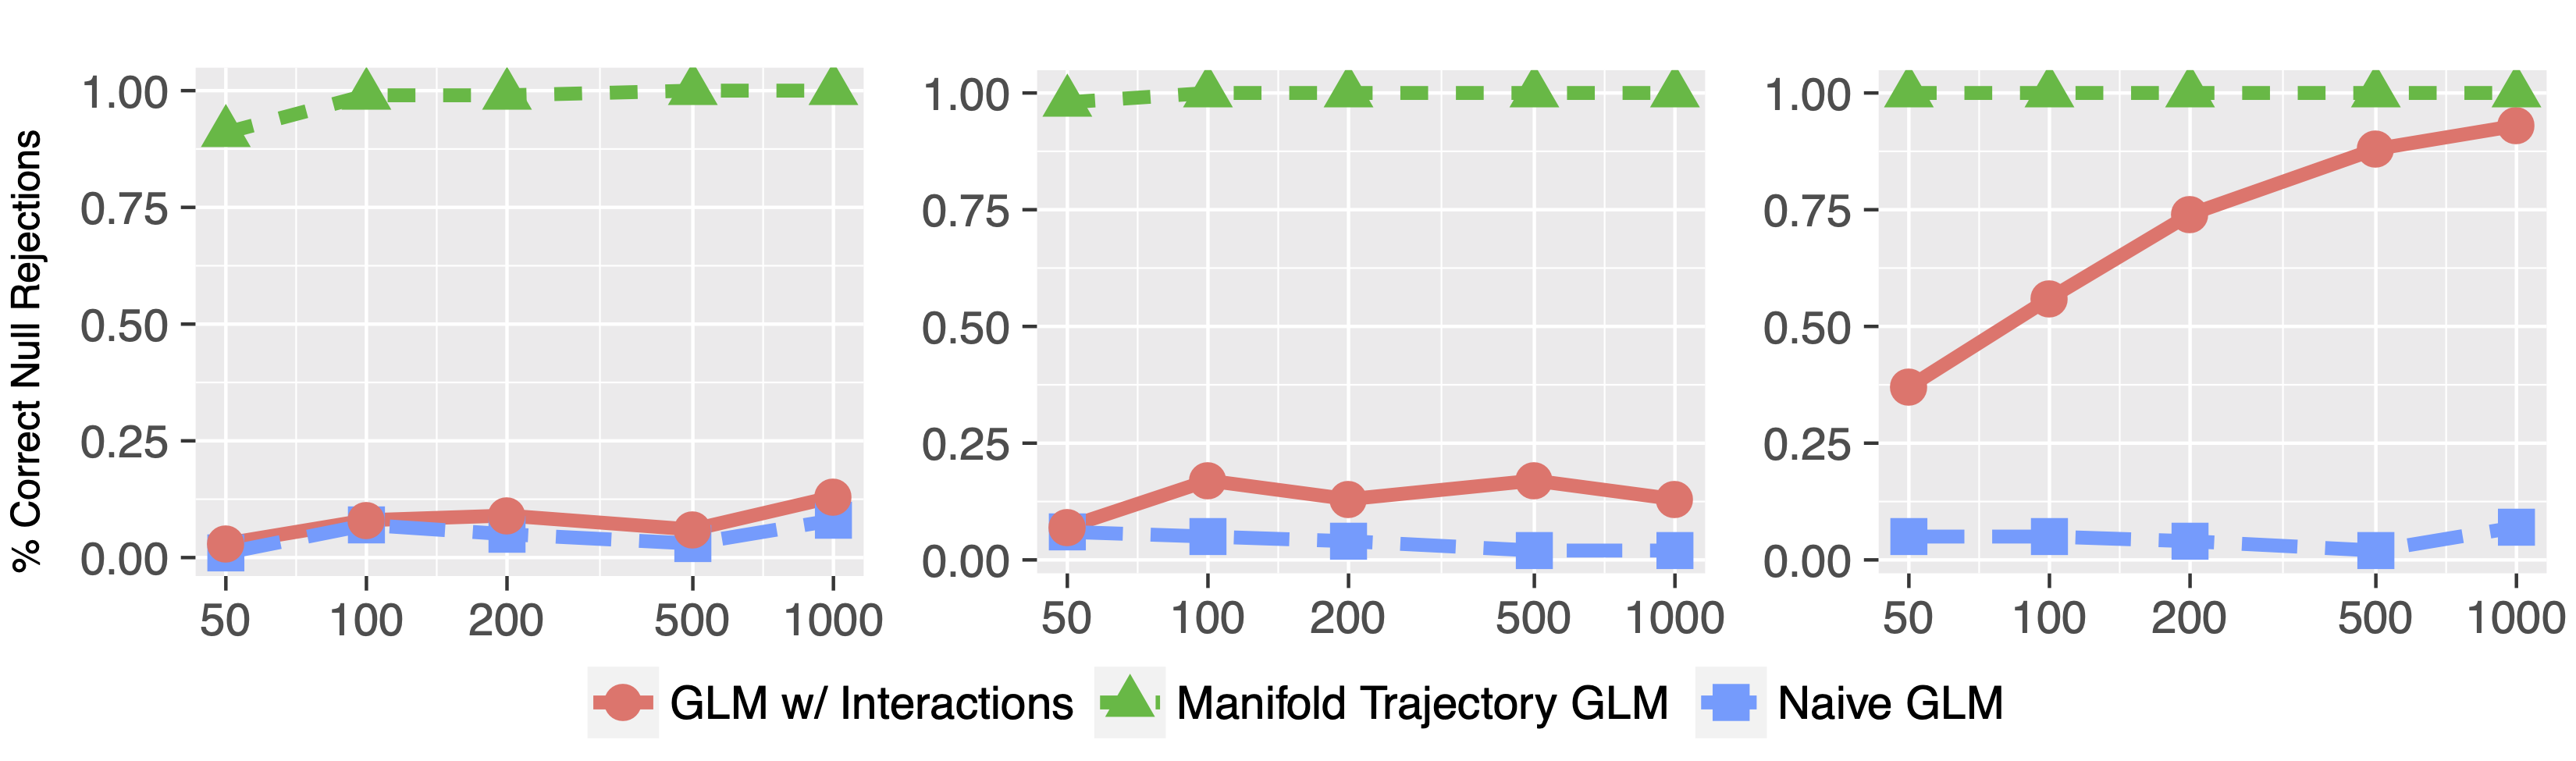
\includegraphics[width=\textwidth]{chap2/sim_results.png}
		\caption{\label{fg:sim_graphs}{\footnotesize Correct null hypothesis rejections over 100 runs for three models. For $p = 50$ features, each plot shows the rejection rate
				for $p_t \in \{4, 8, 20\}$ (from left to right) respectively as a function of the number of sample points.} }
	\end{center}
\end{figure}
%	
Figure \ref{fg:sim_graphs} shows the value of our method over these models. For the interaction GLM case, we randomly select interaction terms to include in the GLM, with size $p_t$ (the ground truth number of variables in the interaction). In this way, we approximate the effect of an oracle specifying to the GLM which terms may describe the underlying interaction. 
We report the fraction of significance tests where a significance threshold 
of $p \leq 0.05$ was found for each model, averaged over 100 runs. 
%Simulated data were generated using the procedure outlined for the simulations above, with more details provided in the Appendix.
We see that our proposed scheme consistently achieves near-perfect results in terms of the percentage of null hypotheses that 
were correctly rejected (i.e., there was a significant group-difference signal). The power of scan statistics on 
graphs is particularly evident in the needle in haystack setting where the true differential signal is small ($p_t \leq 8$)
and the sample size is small to medium. When the sample size is large and $p_t$ is also large, the standard linear model with additional interaction terms starts to approach the statistical performance of our algorithm.



Briefly, we will provide \textbf{(i)} a simple and efficient parametric procedure for modeling temporally evolving graphical models, \textbf{(ii)} a 
hypothesis test for identifying differences between group-wise estimated models, and \textbf{(iii)} a scan
algorithm to identify {\em those subsets of the features which contribute to the group-wise differences}.
Together, these ideas offer a framework for identifying group-wise differences in temporally coupled graphical models.
%We next cover preliminary concepts, we define our model and present an algorithm, followed by experimental results on both simulated data and neuroimaging data 
%acquired from 
From the experimental perspective, we hope to find scientifically plausible results on 
a unique longitudinally tracked cohort of middle-aged (and young elderly) persons at risk for Alzheimer's disease due to family history, 
but who are otherwise completely cognitively healthy.
